\documentclass{article}

%%% IMPORTS %%%
%\usepackage[welsh]{babel}
\usepackage{hyperref}
\usepackage{authblk}
\usepackage{float}
\usepackage{graphicx}
\usepackage[utf8]{inputenc}
\graphicspath{{img/}}


\author[1,3]{Preben Vangberg}
\author[2]{Sondre L. Gjesdal}
\author[3]{Håvard Syslak}

\affil[1]{Department of Computer Science, Aberystwyth University, Wales}
\affil[2]{Western Norway University of Applied Sciences, Norway}
\affil[3]{MMP PM MON MAIN AUT, Equinor ASA, Norway}


%%% DATA %%%
\title{Hacathon Hanes Report and Findings}

%%% DOCUMENT %%
\begin{document}

\maketitle
\newpage

\section{Introduction}

Hacathon Hanes is a hackathon set to be arranged by the National Library of Wales in Aberystwyth Tuesday the 11th of February.
Because of the inability of me (Preben Vangberg) to attend the hackathon in person, I got together with some friends during Saturday the 8th of February to organise a small local version of the Hackathon in Norway.
This report outlines the work we did and shows of some of the findings we were able to make during the session on Saturday.

Of the available datasets, we decided to use Aberystwyth shipping data made available by the National Library.
We went through, filtered, and classified some of the data, in order to produce some results that were interesting to us.

\section{Classification and Filtering of Data}

The field "cause\_of\_leaving" was of some interest to us. The problem we had was that there was approximately 87.000 records, and almost as many causes for leaving. 
We therefore spent a significant amount of time classifying the different reasons for leaving.
These were separated into the following categories: remains on board, discharged, did not join, shipwreck, illness, drowned, deceased, juristical reasons, deserted, transferred, hospitalised, abandoned, transferred, injured, and other. 

These classifications are not perfect and because data is missing, some data is hard to classify, and the semi-manual methodology used, it means that these classifications are approximates. However they still give some insight into the reasons why people left the ship.
There were also so many polite ways of saying that people got injured or died.
This made the classification work harder, as you had to try to understand what 'discharged in the middle of the Atlantic' means for example.
Does this mean that they fell overboard, were thrown overboard, changed ship? This is a lot down to interpretation and trying to make an assumption based on the other data-points. This isn't perfect.

The fields "joined\_ship\_date" and "date\_left", was also of some interest to us.
The issue we had with these fields was that not all fields contained dates, and those that did, not all of the dates where valid (Such as 31. of June).
We therefore wrote a short Python script that filters out entries that contains both a valid "joined\_ship\_date" and "date\_left". This means that a lot of entries which manually could have been fixed, but wasn't. However we managed to get a total of 56842 entries, or around 65\% of the total, which we deemed good enough for our purpose.

It should be noted that we would have wanted to explore different methods and filters, but this is something that can be done on a later date.

\section{Results, Graphs, and Findings}

\subsection{Age Distribution}
\begin{figure}[H]
	\centering
    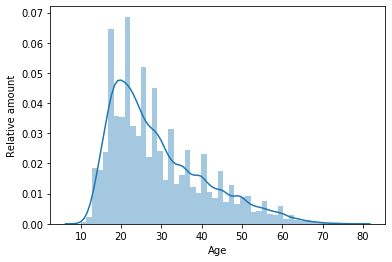
\includegraphics[width=0.9\textwidth]{age}
  	\caption{Age distribution for seamen at the time of joining the ship}
\end{figure}

Based on the graph presented here, we see that the age on-board the ships were quite diverse. The youngest in the dataset was 10, and the oldest was 78 at the time of joining the ship. The curve seems to follow a normal distribution peaking around 20 years old.

\subsection{Classification of Causes of Leaving}

\begin{figure}[H]
	\centering
    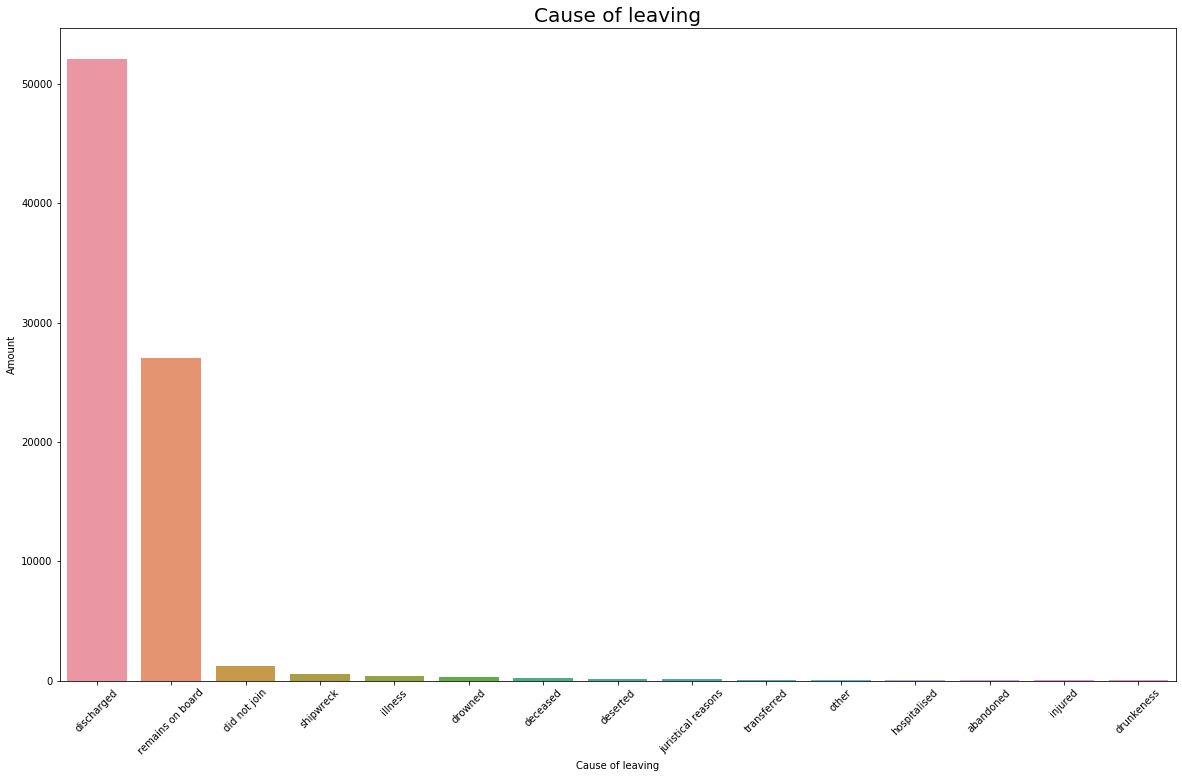
\includegraphics[width=0.9\textwidth]{causes}
  	\caption{Classified causes of leaving}
\end{figure}
\begin{figure}[H]
	\centering
    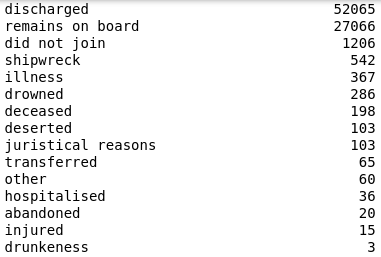
\includegraphics[width=0.9\textwidth]{causes_text}
  	\caption{Classified causes of leaving}
\end{figure}

The majority of the people were discharged. In our definition this is everyone who leaves with mutual consent, retires, is discharged, or has finished service.
There is also a large percentage that remained on-board.
Then we come in to some of the more interesting parts.
\paragraph{Observations:}
\begin{itemize}
	\item 1206 individuals signed up, but never joined the ship. We found this to be much higher than expected.
	\item The category shipwreck involves all loss of ships regardless of whether the crew survived or not.
	\item Juristical reasons is a common category for people who left because of going to jail or being ordered by a court to leave the ship.
	\item Hospitalized is a category for people who were hospitalized for unknown reasons
	\item Transferred means that they were transferred to another ship or job.
	\item Only three persons were thrown of the ship for drunkenness.
\end{itemize}

In general we were surprised of how low some of these numbers were, but they were interesting non the less.
It should also be noted that the work of classifying the data was in itself interesting.
These classifications doesn't show the range of personal stories which we encountered during our classification work and it was these stories which ended up being the most interesting for us.

\subsection{Recruitment, Discharge, and Time On-board}

\begin{figure}[H]
	\centering
    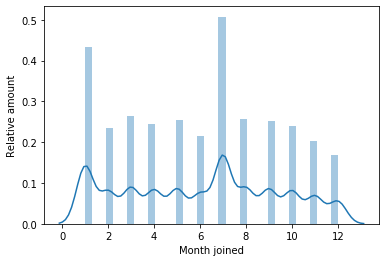
\includegraphics[width=0.9\textwidth]{joined}
  	\caption{Shows which months seamen joined the ship}
\end{figure}

This graph shows which months people joined the different ships and voyages. As you might can see, there is a significant increase in January and July, but there is still some spread evenly throughout the year.

\begin{figure}[H]
	\centering
	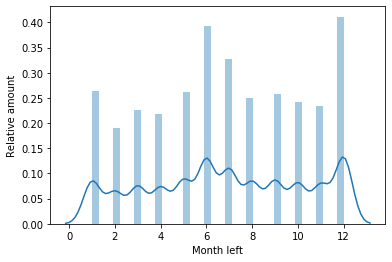
\includegraphics[width=0.9\textwidth]{left_ship}
  	\caption{Shows which months seamen left the ship}
\end{figure}

This graph shows which months people left the ship. There seems to be trend indicating that people return mostly around the end of December/early January and late June/early July.

When we merge these together we can see an interesting picture:

\begin{figure}[H]
	\centering
	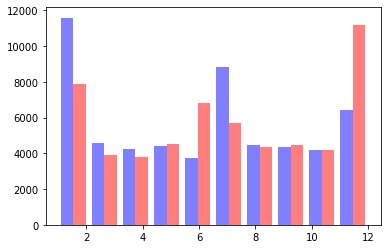
\includegraphics[width=0.9\textwidth]{combi}
  	\caption{Blue: joined, Red: left}
\end{figure}

This seems to indicate that the a lot or most of the crew is discharged in bulks, and hired shortly afterwards. This seems to happen in January and July with 6 months difference.
This intrigued us, which made us graph the time spent on-board. As you can see on the graph below we can also see a spike around 180 days. There is also a spike around 70-90 days. This seems to indicate that a lot of ships tended to be out for 2 to 3 or 6 months at a time, then replacing the crew afterwards.
If we compare this to the shipping-industry today, we can see that this is the case today as well.
A lot of ships today discharges most of their crew and re-hire in set periods (every 6 months for example).

\begin{figure}[H]
	\centering
	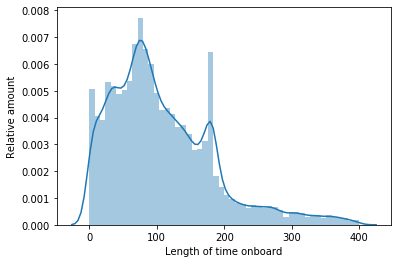
\includegraphics[width=0.9\textwidth]{length}
  	\caption{Time spent at sea}
\end{figure}

\section{Final Thoughs and Conclusions}

Even with the short amount of time, very basic methodologies utilized, and overall simplicity of the resulting data, it was exciting, interesting and educational to work on this data. 
The results were interesting and tell us a bit about the life of seamen in the 19th century.
It would be interesting to see what could be achieved with greater amount of time, more sophisticated methods of classification, and filtering could have produced.
It might be something that can be worth coming back to at a later date.

We would like to thank the National Library of Wales for arranging the hackathon even though we were unable to be there in person.
We had a lot of fun and we learnt a lot of new technologies and libraries which the authors hadn't had much experience in before.
We are definitely looking forward to any other hackathon arranged by the National Library, and we hope to be able to attend these in person.

\end{document}
